\documentclass{beamer}
\usepackage[utf8]{inputenc}
\usepackage{amsthm}
\usepackage{amsmath}
\usepackage{graphicx}
\usetheme{Copenhagen}
\title{Matrix Problem}
\author{Karthik and Abhishek}
\institute{IIT Hyderabad}

\begin{document}
\begin{frame}
\titlepage   
\ 
\end{frame}
\begin{frame}{Contents}
\tableofcontents
\end{frame}
\section{Geometric Question}
\begin{frame}{Geometric Question}
If A is (2,5), B is (4,-11) and C lies on $9x + 7y + 4 = 0$, then the locus of the centroid of triangle ABC is
\end{frame}
\section{Matrix Transformation of Geometric Question}
\begin{frame}{Matrix Transformation Of Geometric Question}
If $\textbf{A}\begin{bmatrix}2 \\ 5\end{bmatrix} and\quad \textbf{B}\begin{bmatrix}4 \\ -11\end{bmatrix}$ are two vertices of a triangle, and the third vertex lies in the line
\\\[\begin{bmatrix}9 & 7\end{bmatrix}\textbf{X} = -4\]
\\Find the locus of the centroid of ABC.
\end{frame}
\section{Solution In Form Of Matrix}
\begin{frame}{Solution In Form Of Matrix}
Consider a parameter t,
\\ \[\textbf{C} = \begin{bmatrix}t \\ (-9t-4)/7\end{bmatrix}\]
\end{frame}
\begin{frame}{Solution In Form Of Matrix}
Finding the Midpoints of BC and AB
\\ Let \textbf{D} be the midpoint of BC, then
\[\textbf{D} = (\textbf{B} + \textbf{C})/2 = \begin{bmatrix}(t+4)/2 \\ (-9t-4-77)/14\end{bmatrix} = \begin{bmatrix}(t+4)/2 \\ (-9t-81)/14\end{bmatrix}\]
\\ Let \textbf{F} be the midpoint of AB, then
\[\textbf{F} = (\textbf{A} + \textbf{B})/2 = \begin{bmatrix}(2+4)/2 \\ (5-11)/14\end{bmatrix} = \begin{bmatrix}3 \\ -3\end{bmatrix}\]
\end{frame}
\begin{frame}{Solution In Form Of Matrix}
Now, Consider $\textbf{N}_1$ to be normal vector to AD, and $\textbf{N}_2$ be normal vector to CF
\\Let \textbf{G} be the centroid.
\\then, \[\textbf{N}_1^T(\textbf{G}-\textbf{A}) = 0\]
\[\Rightarrow \textbf{N}_1^T\textbf{G} = \textbf{N}_1^T\textbf{A}\]
\\and \[\textbf{N}_2^T(\textbf{G}-\textbf{C}) = 0\]
\[\Rightarrow \textbf{N}_2^T\textbf{G} = \textbf{N}_2^T\textbf{C}\]
\end{frame}
\begin{frame}{Solution In Form Of Matrix}
From the equations in the previous slide
\\\[\begin{bmatrix}\textbf{N}_1^T \\ \textbf{N}_2^T\end{bmatrix}\textbf{G} = \begin{bmatrix}\textbf{N}_1^T\textbf{A} \\ \textbf{N}_2^T\textbf{C}\end{bmatrix}\]
\[\Rightarrow \textbf{G} = \begin{bmatrix}\textbf{N}_1^T \\ \textbf{N}_2^T\end{bmatrix}^{-1}\begin{bmatrix}\textbf{N}_1^T\textbf{A} \\ \textbf{N}_2^T\textbf{C}\end{bmatrix}\]
\\On substituting we get
\[\textbf{G} = \begin{bmatrix}(t+6)/3 \\ (-9t-46)/21\end{bmatrix}\]
\end{frame}
\begin{frame}{Solution In Form Of Matrix}
Simplifying,
\[\textbf{G} = 1/21\begin{bmatrix}7(t+6) \\ (-9t-46)\end{bmatrix}\]
\[\begin{bmatrix}9/7 & 1\end{bmatrix}\textbf{G} = 1/21\begin{bmatrix}9/7 & 1\end{bmatrix}\begin{bmatrix}7(t+6) \\ (-9t-46)\end{bmatrix}\]
\[\begin{bmatrix}9/7 & 1\end{bmatrix}\textbf{G} = (1/21)(8)\]
\[\begin{bmatrix}9 & 7\end{bmatrix}\textbf{G} = 8/3\]
\\Therefore locus is a straight line
\[\begin{bmatrix}27 & 21\end{bmatrix}\textbf{X} = 8\]
\\Locus in cartesian form is
\[27x + 21y = 8\]
\end{frame}
\begin{frame}{Figures}
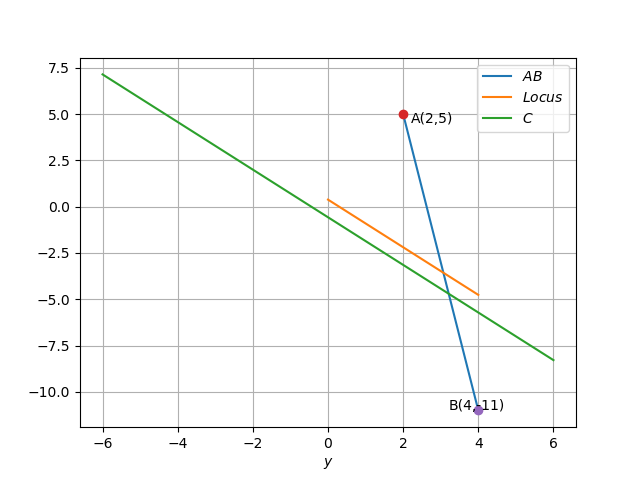
\includegraphics[scale = 0.6]{locus.png}
\end{frame}
\begin{frame}{Figures}
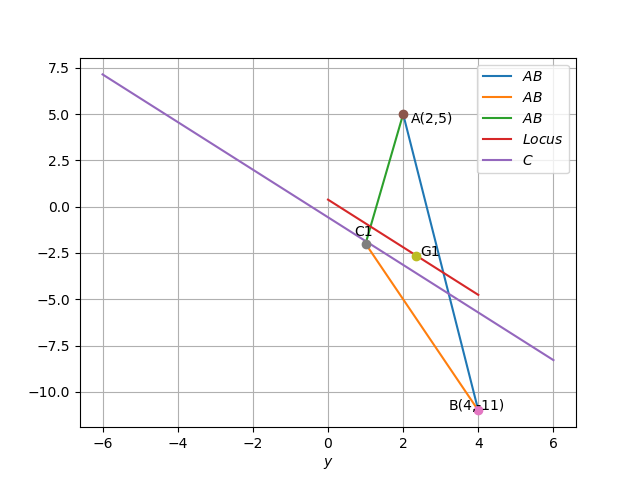
\includegraphics[scale = 0.6]{triangle.png}
\end{frame}
\end{document}